\subsubsection{Fine-tuning on small clinical datasets}

We assessed the generalizability of our baseline model by fine-tuning it on small datasets from four institutions that may use different surgical approaches and acquisition protocols (including contrast enhancement and anisotropic spacing in \textit{Strasbourg}) (\cref{sec:multicenter}).
Additionally, we fine-tuned the model on 20 cases from EPISURG with the lowest \ac{DSC} in \cref{sec:self}.

For each dataset, we load the pretrained baseline model, initialize the optimizer with an initial learning rate of $5 \times 10^{-4}$, initialize the learning rate scheduler and fine-tune all layers simultaneously for 40 epochs using 5-fold cross-validation.
We use model weights from the epoch with the lowest mean validation loss for evaluation.
To minimize data leakage, we determined the above hyperparameters using the validation set of one fold in the \textit{Milan} dataset.

We observed a consistent increase in \ac{DSC} for all fine-tuned models, up to a maximum of 89.2 (13.3) for the \textit{Milan} dataset.
For comparison, inter-rater agreement between human annotators in our previous study was 84.0 (9.9) \cite{perez-garcia_simulation_2020}.
Quantitative and qualitative evaluations are illustrated in \cref{fig:finetuning_quant,fig:finetuning_qual}, respectively.


\begin{figure}
  \centering
  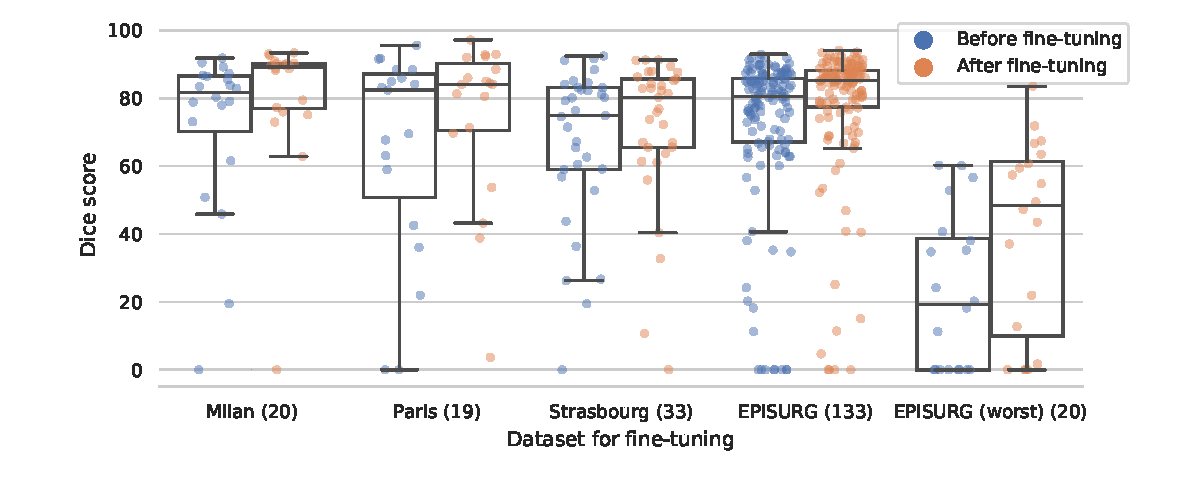
\includegraphics[trim=1cm 0 0.8cm 0, clip, width=\linewidth]{boxplot_finetuning}
  \caption[Dice score without before and after fine-tuning]{
    \ac{DSC} without (blue) and with (orange) fine-tuning of the model training using self-supervision.
    Horizontal lines in the boxes represent the first, second (median) and third quartiles.
    The `EPISURG (worst)' dataset comprises the 20 cases from EPISURG with the lowest \ac{DSC} in the experiment described in \cref{sec:self}.
    Numbers in parentheses indicate subjects per dataset.
  }
  \label{fig:finetuning_quant}
\end{figure}


\begin{figure}[ht!]
  \centering
  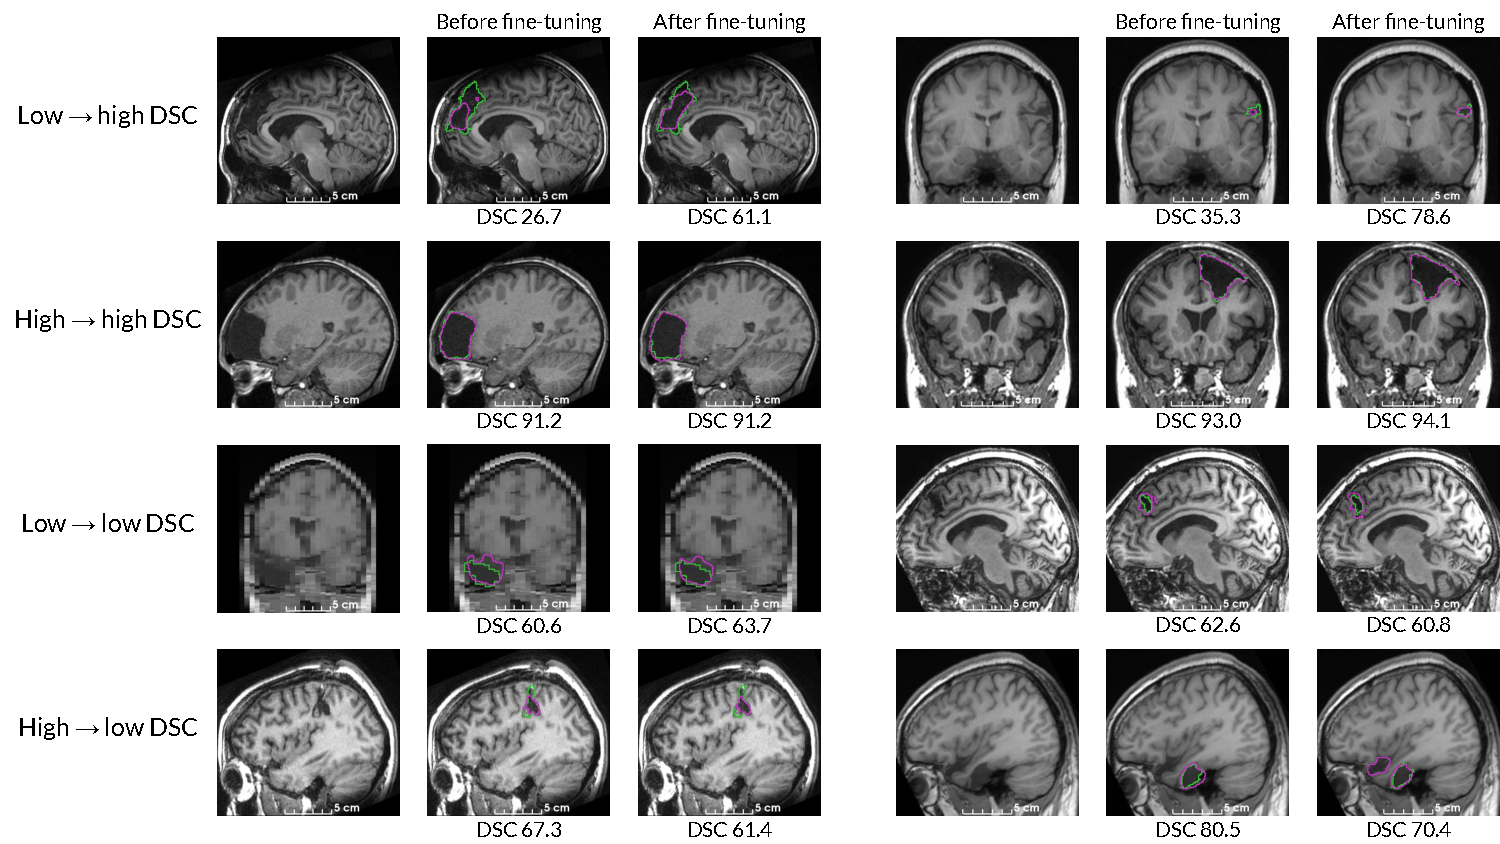
\includegraphics[width=\linewidth]{finetune}
  \caption[Qualitative evaluation of fine-tuning]{
    Qualitative evaluation of fine-tuning for the \textit{Strasbourg} (left) and EPISURG (right) datasets.
    Rows correspond, from top to bottom, to cases for which the \ac{DSC}
    1) increased,
    2) remained high,
    3) remained low and
    4) decreased
    after fine-tuning the self-supervised model.
    Manual annotations (green) and model predictions (magenta) are overlaid.
  }
  \label{fig:finetuning_qual}
\end{figure}
